\documentclass[12pt,titlepage,a4paper]{report}

% Texte
\usepackage[utf8]{inputenc}
\usepackage[T1]{fontenc}
\usepackage[french]{babel}
\usepackage{lmodern}
\usepackage{array}

% Numéroter les chapitres a partir de chaque début de partie
\makeatletter\@addtoreset{chapter}{part}\makeatother

% Mise en page
\usepackage{url}
\usepackage[top=2.1cm,bottom=2cm,left=1cm,right=1cm]{geometry}
\usepackage{hyperref}
\hypersetup{
    colorlinks=false,
    pdfborder={0 0 0},
}
\usepackage{multirow}

% TOC
\usepackage[french]{minitoc}
\setcounter{tocdepth}{0}
\setcounter{minitocdepth}{2}
\setlength{\mtcindent}{0pt}

% Images
\usepackage{float}
\usepackage{wrapfig}
\usepackage{graphicx}
% Pour inclure des pages PDF
\usepackage[final]{pdfpages}

% Couverture
\usepackage{templateINSA}
\initINSA

\title{Projet d'électronique}
\author{Antoine \bsc{Augusti}\\ Etienne \bsc{Batise}\\ Jean-Claude \bsc{Bernard}\\ Thibaud \bsc{Dauce}}

\renewcommand\soustitre{Un réveil intelligent}
\renewcommand\infoBig{Projet d'électronique}
\renewcommand\infoSmall{ASI3 2013-2014}

\def\changemargin#1#2{\list{}{\rightmargin#2\leftmargin#1}\item[]}
\let\endchangemargin=\endlist 

\begin{document}
	\titleINSA{15}{images/fond.jpg}{0}{0}{300}{\href{http://www.flickr.com/photos/lord_james/4696338852/sizes/o/in/photostream/}{\textcolor{white}{Licence CC - Lord James}}}

	\dominitoc
	\tableofcontents

	\setcounter{page}{1}
	\part{TODO}
	un couverture explicite : photo, noms des élèves et du prof, classe année titre projet

	un CD-Rom contenant les fichier pdf du dossier complet, le cahier de suivi, les photos, les vidéos, les liens internet, le bon de commande

	
	\part{Introduction}
	\chapter{État de l'art}
	\minitoc
	\section*{Introduction} % (fold)
\label{sec:introduction}
\addcontentsline{toc}{section}{Introduction}

Dans le cadre de notre première année de cycle ingénieur dans le département ASI\footnote{ASI : Architecture des Système d'Information}, nous avons pour mission de réaliser pour le cours d'Électronique pour l'ingénieur dispensé par Monsieur \bsc{Henriet} un projet d'une durée de 6 mois en rapport avec le domaine de l'électronique. Une partie de notre groupe ayant réalisé un robot auparavant dans le cadre du projet de P6, nous avons choisis de découvrir ensemble de nouvelles technologies de façon à agrandir notre vision dans ce domaine.\\

Notre attention s'est très rapidement portée sur l'un des projet déjà réalisé par un groupe d'étudiant l'année dernière : \emph{Un réveil intelligent}. En effet, ce projet est véritablement dans la vague des nouvelles technologies domotiques qui deviennent de plus en plus populaires. C'est pourquoi nous nous sommes fixés comme but d'améliorer ce projet par de nouvelles fonctionnalités. \\

Malgré la réussite de ce projet, il est néanmoins indispensable d'effectuer pour nous un état de l'art sur les différents caractéristiques actuelles du projet d'une part, et de nos projets d'autres part. C'est pourquoi dans ce dossier nous allons d'abord vous parler des différents modèles de carte à programmer telles que les Arduino ou les Raspberry Pi. Ensuite nous présenterons les différents langages de programmation à utiliser et leur utilité. Enfin nous expliquerons quels nouveaux types de matériel nous allons utiliser pour arriver à notre but.\\

% section introduction (end)
\section{Les différents modèles de Raspberry} % (fold)
\label{sec:les_diff_rents_mod_les_de_raspberry}

\subsection{Qu'est-ce qu'un Raspberry ?} % (fold)
\label{sub:qu_est_qu_un_raspberry}
Un Raspberry, ou pour son nom complet un Raspberry Pi, est une mini-ordinateur, de la taille d'une carte de crédit, tournant avec un processeur ARM. Un processeur ARM est du même type que ceux que l'on trouve dans nos tablettes ou smartphone, leur principale caractéristique est leur faible consommation d'énergie. Le Raspberry Pi est composé uniquement d'une carte mère sans boitier, sans alimentation ni stockage mais il possède un grand nombre d'entrées sorties dites standards. Les plus importantes sont : un lecteur de carte SD (pour le stockage), un prise HDMI (afin de le connecter à un écran), un ou des ports USB (afin en particulier de pouvoir y brancher un clavier et / ou une souris mais aussi des clés USB ou d'autres périphériques USB tel que un dongle Wi-Fi). \\

\begin{figure}[h]
  	\centering
  	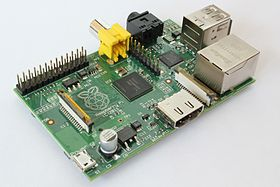
\includegraphics[scale= 0.6]{images/RaspberryPi.jpg}
  	\caption{Raspberry Pi}
\end{figure}

Le principal problème de ce mini-ordinateur est qu'il est alimenté en USB (5 Volts) ce qui explique le choix d'un processeur ARM, peu gourmant en énergie certe, mais peu puissant en contrepartie. Cette faible alimentation est aussi un problème concernant les périphériques USB. Par exemple, un clavier rétro-éclairé peut consommer trop d'énergie et rendre le Raspberry Pi défaillant. \\

Toutefois le Raspberry Pi possède de nombreux avantages. En premier lieu, il est capable de faire tourner un système d'exploitation de type GNU / Linux très puissant et permettant d'effectuer des tâches très variées. Il est en effet possible d'installer sur un Raspberry Pi un serveur web (de type Apache), un serveur mail, un système de partage de fichier (type Samba) ou encore une seedbox (afin de partager des fichiers torrent). Là où l'alimentation était un problème, sa faible consommation devient un avantage si il reste allumé 24h / 24 7j / 7. Ce mini-ordinateur se distingue aussi par ses incroyables capacités graphique car malgré un processeur peu puissant, il arrive a décoder des vidéos full HD (1080p) sans aucun problème. Il est souvent utilisé comme \textit{media center}, branché à une télévision et au réseau, permettant ainsi de regarder des films stockés sur son ordinateur facilement. \\

Pour finir, le prix du Raspberry d'environ 30 euros le rend très attractif aux vues de ses capacités très vastes. Il peut être intégré dans de nombreux projets de robotique allant du ballon sonde à un serveur de domotique.\\
% subsection qu_est_qu_un_raspberry (end)

\subsection{Deux grands types de Raspberry Pi} % (fold)
\label{sub:deux_grands_types_de_raspberry_pi}
Il existe deux types de Raspberry Pi : le modèle A et le modèle B. Le modèle B se distingue de son homologue moins cher sur plusieurs points : une RAM plus importante (512 Mo au lieu de 256 Mo), un port USB supplémentaire, un port Ethernet 10/100 et une meilleure puissance électrique (700mA au lieu de 400mA). \\

Pour notre projet, nous n'avons pas le choix du Raspberry Pi car nous allons reprendre celui utilisé pour le projet de P6 du "Réveil intelligent". C'est un modèle B muni donc d'un port Ethernet mais malheureusement plus vieux que l'actuelle version donc n'aillant quand même que 256 Mo de RAM. Si nous avions dû choisir, c'est ce modèle plus performant que nous aurions prit en grande partie pour son port Ethernet permettant des applications réseau mais aussi pour ses meilleures performances d'alimentation qui pourront nous être utile dans le futur.\\

Nous tenons à lever un problème du Raspberry Pi modèle B, les deux ports USB et le port Ethernet sont reliés au même composant "LAN9512" qui est lui-même connecté au CPU via un port USB2 : les débits sont donc divisés entre les trois éléments. Dans notre cas, ce n'est pas un problème car nous ne comptons pas effectuer des transferts importants de données en USB ou en réseau.\\ 
% subsection deux_grands_types_de_raspberry_pi (end)

\subsection{La carte Arduino} % (fold)
\label{sub:la_carte_arduino}
Arduino est un circuit imprimé possédant un microcontrôleur lui permettant d'analyser des signaux électriques. Ce composant est déjà présent dans le projet que nous comptons reprendre et nous pouvons donc le réutiliser. \\

\begin{figure}
  	\centering
  	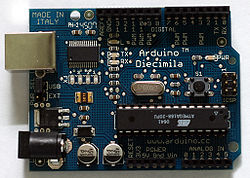
\includegraphics[scale= 0.6]{images/Arduino.jpg}
  	\caption{Carte Arduino}
\end{figure}

Contrairement à un Raspberry Pi, la carte Arduino possède un grand nombre d'entrées / sorties (une vingtaine alors que le Raspberry Pi en possède uniquement 6) mais ne peut pas exécuter de système d'exploitation et donc de programme en temps que tel. Le microcontrôleur peut quand même effectuer des calculs qui seront développés en C / C++. Le dernier point intéressant sur la Arduino est de pouvoir recevoir des signaux analogiques alors que le Raspeberry Pi ne peut lire que des signaux numériques, il aura donc en charge de transformer les signaux analogiques des capteurs (luminosité par exemple) en numérique (0 ou 1 en fonction d'un seuil). \\
% subsection la_carte_arduino (end)

% section les_diff_rents_mod_les_de_raspberry (end)
\section{Les différents langages} % (fold)
\label{sec:les_diff_rents_langages}
Nous allons être amenés à utiliser plusieurs langages de programmation bien différents les uns des autres pour pouvoir réaliser ce projet. La séparation la plus marquée pour ces langages peut se faire par leur but : une partie des langages sera utilisée pour l'intelligence de nos applications, tandis que les autres langages seront dédiés à la création d'une IHM\footnote{IHM : Interface Homme Machine}.

\subsection{Les langages dédiés à l'intelligence de notre application}
La logique métier et les différentes fonctions de notre application seront écrites en PHP\footnote{PHP : \textit{PHP Hypertext Preprocessor}.} et en script shell.\\

PHP est un langage de programmation compilé à la volée libre principalement utilisé pour produire des pages Web dynamiques via un serveur HTTP, mais pouvant également fonctionner comme n'importe quel langage interprété de façon locale. Le langage PHP permettra de programmer les différentes fonctions de notre application ainsi que de stocker et d'aller chercher les données utiles à son fonctionnement.\\

Les scripts shell (également appelés scripts bashs) permettent d'automatiser une série de commandes exécutées dans un terminal. Un script shell se présente sous la forme d'un fichier contenant une ou plusieurs commandes qui seront exécutées de manière séquentielle. Ces scripts nous permettront d'automatiser des opérations de maintenance, de mises à jour ou de modifications de notre Raspberry.

\subsection{Les langages dédiés à la création de l'IHM}
L'Interface Homme Machine de notre application sera accessible depuis un navigateur web (Firefox ou Google Chrome par exemple). Pour pouvoir proposer une IHM accessible depuis un navigateur web, il est obligatoire d'utiliser les langages associés au monde du web à savoir HTML\footnote{HTML : \textit{Hypertext Markup Language}.} et CSS\footnote{CSS : \textit{Cascading Style Sheets}}. Nous utiliserons également du JavaScript pour pouvoir proposer une interface plus dynamique.\\

Le HTML est le format de données conçu pour représenter les pages web. C'est un langage de balisages qui permet d'indiquer qu'un élément est un titre, un paragraphe, un lien, une liste, un élément d'une liste etc.\\

Le feuilles de style CSS, quand elles sont associées à du HTML, permettent de mettre en forme une page web en spécifiant comment sont positionnés les éléments, quelles couleurs il faut utiliser, quels sont les tailles et espaces à respecter. Le CSS définit l'aspect graphique de la page web tandis que le HTLM ne s'occupe que de la sémantique du contenu de celle-ci.\\

Le JavaScript (souvent abrégé JS) est un langage de programmation de scripts principalement utilisé dans les pages web interactives mais aussi côté serveur. Il permet de modifier des pages web quand un événement est déclenché (le survol d'un élément, un délai dépassé, une position atteinte etc.) sans devoir rafraîchir celle-ci, donnant la possibilité d'avoir des modifications instantannées à l'écran dès qu'une action de la part de l'utilisateur est effectuée. Le JavaScript est capable de modifier du CSS et du HTML.

% section les_diff_rents_langages (end)



\section{Les choix de la source de lumière} % (fold)
\label{sec:les_choix_de_la_source_de_lumi_re}
	
% \subsection{Le choix de l'ampoule}
	
On trouve trois grandes familles d'ampoules : les lampes à incandescences, les sources à décharge luminescentes pressurisées et les sources électroluminescentes.
	
\begin{wrapfigure}{r}{25mm}
  	\centering
  	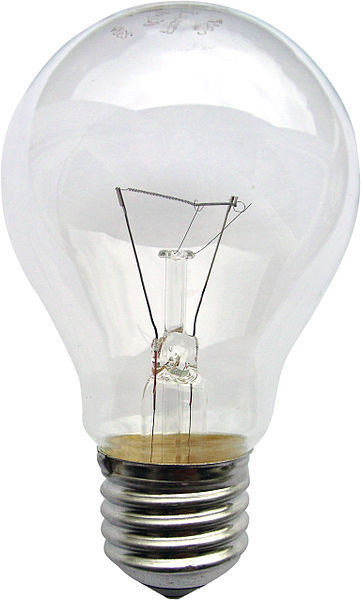
\includegraphics[scale= 0.2]{images/incandescence.jpg}
  	\caption{Ampoule à incandescence}
\end{wrapfigure}
	
La lampe à incandescence classique, inventée en 1879 par Joseph Swan et améliorée par les travaux de Thomas Edison, ou à halogène, inventée en 1959, produit de la lumière en portant à incandescence un filament de carbone (à l'origine) ou de tungstène.\\
	
Ensuite, on a les sources à décharge luminescentes pressurisées telles que les lampes fluorescentes compactes. Celles-ci produisent de la lumière grâce à un mélange de gaz et/ou de vapeur excité par une décharge électrique. Contrairement aux lampes à incandescences, on a une plus grande luminosité (jusqu'à 115 lumens par watt) et le coût est similaire. Toutefois l'allumage n'est pas instantané.\\
		
Enfin, les lampes électroluminescentes sont constituées d'un matériau semi-conducteur traversé par un courant électrique et émettent une couleur bleue. Par des procédés chimiques, on va pouvoir convertir la lumière en jaune. Ces types de lampes ont la plus grande longévité et chauffent beaucoup moins que les lampes à incandescences. Néanmoins, ce sont les ampoules les plus chères du marché actuellement. \\

\section*{Conclusion} % (fold)
\label{sec:conclusion}
\addcontentsline{toc}{section}{Conclusion}
	Après avoir établi un état de l'art des différents outils et technologies que nous allons utiliser, nous avons donc de bonnes bases pour commencer à nous organiser et nous lancer réellement dans la conception globale du projet.
% section conclusion (end)


	\part{Cahier des charges}
	\chapter{Cahier des charges}
	\section{Électronique} % (fold)
\label{sec:_lectronique}

\begin{itemize}
	\item Faire un circuit imprimé pour remplacer le shield actuel
	\item Implémenter un système d'ampoule
	\item Implémenter une alimentation autonome
	\item Effectuer tous les branchements 
\end{itemize}
\vspace{20px}

Le shield existant permet, grâce à une photorésistance, de déterminer la luminosité dans la pièce où se situe le réveil. Il est fonctionnel mais nous devons créer notre propre carte pour répondre aux besoins du projet. Cette carte aura les même objectifs que le shield, c'est-à-dire retourner une valeur analogique en fonction de la luminosité de la pièce. L'ancien shield possède une LED, contrôlée par la Arduino, permettant de savoir quand la luminosité dépasse un certain seuil. Pour notre projet, nous comptons intégrer le réveil dans une boite et nous pensons réutiliser la LED afin de prévenir l'utilisateur que la batterie du réveil est faible. \\

Nous devons choisir l'ampoule et la connecter à notre circuit imprimé afin de pouvoir contrôler la quantité de courant à envoyer et ainsi proposer un éclairage progressif. \\

Le dernier objectif de cette partie d'électronique est d'effectuer des montages et par extension des câblages propres afin de produire un travail de qualité et de faciliter l'intégration des différentes cartes dans un boitier. \\

% section _lectronique (end)

\section{Arduino} % (fold)
\label{sec:arduino}

\begin{itemize}
	\item Implémentation de la gestion de l'ampoule
	\item Réutiliser la LED pour signaler que la batterie est faible 
\end{itemize}
\vspace{20px}

Au niveau de la Arduino, le code présent permet déjà de déterminer lorsque le seuil de luminosité est dépassé. Il nous faudra donc ajouter l'allumage progressif de l'ampoule. Nous devrons aussi résoudre les conflits entre l'allumage de l'ampoule et le capteur de luminosité afin de ne pas précipiter l'arrêt du réveil. Nous pourrons pour cela adapter le code déjà produit par l'équipe précédente et implémenter, par exemple, une variation du seuil de luminosité en fonction du stade d'allumage de l'ampoule. \\

La gestion de la batterie est importante et nous devrons trouver un moyen de déterminer quand le niveau de batterie du réveil est faible pour pouvoir prévenir l'utilisateur (afin de ne pas se retrouver sans réveil du jour au lendemain). À ce stade de la conception, nous ne savons toujours pas si cette information pourra être récupérée directement via la Arduino ou si (plus probablement) nous devrions récupérer certaines informations via notre circuit imprimé. Cette batterie va nous permettre d'alimenter le Raspberry Pi et la Arduino sans câble, si nous voulons un boîtier autonome nous avons aussi besoin de supprimer le câble RJ-45 permettant l'accès au réseau. Nous devons donc rajouter un dongle Wi-Fi qui peut consommer très rapidement beaucoup de courant. Il faut donc aussi implémenter une gestion du Wi-Fi : bouton on / off ou allumage intelligent (un peu avant le déclenchement du réveil par exemple). \\

% section arduino (end)

\section{Raspberry Pi} % (fold)
\label{sec:raspberry_pi}

\begin{itemize}
	\item Affichage des prochains métros
	\item Gestionnaire de sons
	\item Implémentation de l'affichage LCD
	\item Paquet magique sur le réseau (broadcast) 
\end{itemize}
\vspace{20px}

L'affichage des prochains métro semble ne pas fonctionner actuellement sur le projet, sans doute à cause d'un changement sur le site de la TCAR. Il nous faudra réparer cette fonctionalité. \\

Au niveau des améliorations, il n'existe pas de gestionnaire de son sur l'interface web permettant l'administration du réveil et donc, le changement de la sonnerie du réveil est laborieux. Nous comptons implémenter une nouvelle page web permettant d'ajouter des nouveaux sons et de choisir celui à jouer au prochain réveil. \\

Les deux dernières fonctionnalités sont optionnelles, même si nous aimerions les implémenter, il est peu probable que nous ayons le temps vu les délais à respecter pour le projet. La première consiste à gérer l'affichage de l'heure via un écran LCD et la deuxième, un peu plus technique mais très utile, permettrait d'envoyer un paquet "magique" TCP / IP sur le réseau local de l'utilisateur lors de la sonnerie du réveil (et pourquoi pas lors de son extinction) afin de donner la possibilité de réutiliser ce projet. En effet, un paquet "magique" est un paquet qui peut être lu par tous les appareils connectés au réseau, cela donne donc la possibilité de créer un autre projet d'électronique (par exemple un autre Raspberry Pi) analysant le réseau et exécutant une action lors de la détection de ce paquet (par exemple, allumage de l'ordinateur, de la cafetière ou autre\dots). \\

% section raspberry_pi (end)

\section{Bricolage} % (fold)
\label{sec:bricolage}

\begin{itemize}
	\item Construire une boîte 
\end{itemize}
\vspace{20px}

Il ne faut pas oublier de prendre le temps de construire une boîte afin de protéger les circuits et rendre le projet plus esthétique. \\

% section bricolage (end)


	\part{Étude technique}
	\chapter{Électronique}
\minitoc

\section{La lumière : Shield LDR}
\subsection{Schéma du Shield LDR}
\begin{figure}[h]
	\centering
	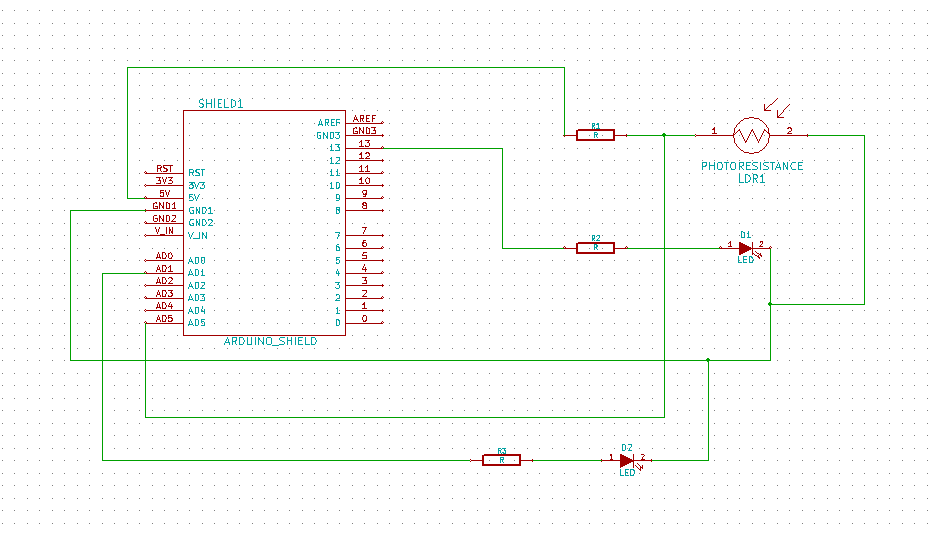
\includegraphics[width=550px]{images/SchemaElectriqueShield.png}
	\caption{Logiciel utilisé : Eeschema de Kicad}
\end{figure}

\subsection{Choix des composants} 
	Notre projet étant une reprise d'un projet de l'année dernière, nous avons dû refaire le shield. Nous avons donc récupéré leurs composants à savoir :
	\begin{itemize}
		\item Une Arduino Mega 2560
		\item Deux LEDs 
		\item Une photorésistance LDR
		\item Trois résistances
	\end{itemize}

\section{Alimentation autonome : 7805}
\subsection{Schéma du régulateur de tension}
\begin{figure}[h]
	\centering
	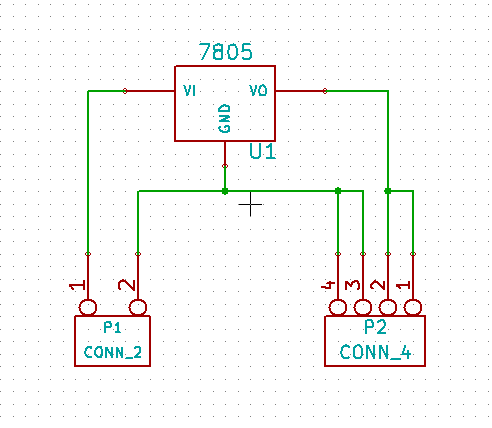
\includegraphics[width=350px]{images/SchemaDuRegulateur.png}
	\caption{Logiciel utilisé : Eeschema de Kicad}
\end{figure}

\subsection{Choix des composants} 
	Nos camarades de l'année dernière alimentaient leurs Arduino et Raspberry avec une prise secteur. Cette année, nous avons décidé d'en faire un réveil portable. Et qui dit portable, dit alimentation autonome. Les deux appareils étant alimentés en 5V, nous avons commandé un régulateur de tension 7805 qui délivre du 5V/1A. On met donc en entrée du régulateur un pack d'accus de 7V et le régulateur va se charger de délivrer du 5V à l'Arduino et à la Raspberry branchées en dérivation sur celui-ci.

\section{Communication Arduino-Raspberry}
	Comme la Arduino reçoit les informations du capteur de luminosité et allume la lampe, et que le Raspberry est en charge du réveil, il a fallu établir une communication entre les deux cartes. Pour cela nous utilisons deux pins du Raspberry et deux pins du la Arduino afin de pouvoir envoyer et recevoir des informations grâce à une liaison bi-directionnelle.\\

	D'un côté, le Raspberry va envoyer un signal de réveil à la Arduino afin qu'elle puisse commencer à allumer la LED. Et inversement, lorsque que la Arduino détecte une source de lumière, elle envoie un signal au Raspberry afin qu'il puisse éteindre la sonnerie du réveil.


	\part{Documents de réalisation}
	\chapter{Calendrier prévisionnel}
	Retrouvez ci-dessous le calendrier prévisionnel de la réalisation de notre projet.
	\begin{center}
	\begin{tabular}{| l | m{3.5cm} | m{3.5cm} | m{3.5cm} |}
		
		\hline
		\textbf{Dates} & \textbf{Électronique} & \textbf{Arduino} & \textbf{Raspberry Pi} \\ \hline
		25/09/2013 & Determiner le travail à fournir & Prendre en main le logiciel Arduino & Découvrir l'interface RaspberryPi \\ \hline
		
		09/10/2013 & Remplacer le Shield Arduino par une carte PCB & Commencer le développement de la gestion de l'ampoule & \\ \hline
		
		23/10/2013 & Ajouter une ampoule au montage et trouver une solution pour une alimentation autonome	& Effectuer les tests de la gestion de l'ampoule & \\ \hline
		
		13/11/2013 & Implémentation de l'alimentation autonome & Développer un indicateur de la charge restante de la batterie & Commencer le développement du gestionnaire de métros \\ \hline
		
		27/11/2013 & Effectuer et vérifier tous les branchements définitevement & & Commencer le développement du gestionnaire de sons\\ \hline
		
		11/12/2013 & & & Commencer la gestion d'un affichage sur écran LCD \\ \hline
		
	\end{tabular}
\end{center}
	
	\chapter{Cahier de suivi}
	\minitoc
	Retrouvez ci-dessous le cahier de suivi de notre projet.
	\documentclass[a4paper, 12pt, french]{article}

\usepackage[utf8]{inputenc} 	%package pour le français sous ubuntu : à vous d'adapter
\usepackage[french]{babel}	%pour le français
\usepackage[T1]{fontenc}	%pour les polices
\usepackage{fullpage}

\title{Cahier de suivi}
\author{Antoine Augusti\\ Etienne Batise\\ Jean-Claude Bernard\\ Thibaud Dauce}

\begin{document}
\maketitle

	\section*{Mercredi 13 Novembre 2013 } % (fold)
	\label{sec:mercredi_13_octobre_2013 }
	\begin{itemize}
		\item Tests concluants du code arduino pour l'allumage progressif de l'ampoule
		\item Finalisation des cartes réalisation des typons sur papier non transparent
		\item Recherche des méthodes de gestion de batterie pour RaspberryPi
	\end{itemize}

	% section mercredi_13_novembre_2013 (end)

	\section*{Mercredi 23 Octobre 2013 } % (fold)
	\label{sec:mercredi_23_octobre_2013}
	\begin{itemize}
		\item Début débugage du parsing des métros 
		\item Premiers tests du nouveau code (allumage progressif d'une LED)
		\item Premiers tests d'intégration d'une LED dans le circuit.
	\end{itemize}
	
	% section mercredi_23_octobre_2013 (end)

	\section*{Mercredi 09 Octobre 2013} % (fold)
	\label{sec:mercredi_09_octobre_2013}
	\begin{itemize}
		\item Développement du programme Arduino. À faire : les tests.
		\item Le shield actuel a été refait et validé. Il reste à monter la nouvelle ampoule dessus.
		\item Recherches sur l'ampoule ainsi que sur la méthode d'alimentation autonome(Batterie Li-Po x2, Régulateur de tension 7805, cartes montées en parallèles et ampoules 4,8V)
		\item
	\end{itemize}
	% section mercredi_09_octobre_2013 (end)

	\section*{Mercredi 25 Septembre 2013} % (fold)
	\label{sec:mercredi_25_septembre_2013}
	\begin{itemize}
			\item Prise en main de l'interface du RaspberryPi. Beaucoup de problème avec le réseau INSA (proxy vs serveur local)
			\item Prise en main de l'arduino et lecture du code.
			\item Définition des objectifs à atteindre du point du vue électronique..
	\end{itemize}	
	% section mercredi_25_septembre_2013 (end)
\end{document}



	\part{Étude logicielle}
	\chapter{Raspberry}
	\minitoc
	\section{Réseau}
	Le principal problème que nous avons rencontré était au niveau de la gestion des contraintes réseau : nous avions besoin d'utiliser le serveur local du Raspberry pour proposer l'interface web de configuration du réveil et un accès au web complet pour proposer des services extérieurs : les prochains métros, la météo et les news.\\

	Pour nous connecter au web nous avions à notre disposition dans les salles de TP le réseau de l'INSA qui oblige à passer par le proxy\footnote{En informatique, un proxy est un composant logiciel qui joue le rôle d'intermédiaire en se plaçant entre deux autres pour faciliter ou surveiller leurs échanges.

	Dans le cadre plus précis des réseaux informatiques, un proxy est alors un programme servant d'intermédiaire pour accéder à un autre réseau, généralement internet. Par extension, on appelle aussi proxy un matériel (un serveur par exemple) mis en place pour assurer le fonctionnement de tels services.} de l'INSA pour atteindre le web.\\

	Malheureusement l'utilisation du proxy de l'INSA est incompatible avec l'utilisation d'un serveur local simultanément. Pour pouvoir utiliser ces deux services simultanément nous avions besoin de spécifier des règles de proxy spécifiques et supplémentaires par rapport à ce que le proxy de l'INSA propose naturellement. Une fois la solution trouvée, nous avons alors créé un fichier de configuration pour le proxy répondant à notre besoin.\\

	Enfin, le navigateur web proposé par défaut sur Raspberry n'étant pas capable de lire ce type de fichier de configuration, nous avons téléchargé le navigateur web Chromium.

\section{Gestionnaire de sons}
	Pour être efficace, notre réveil devait jouer un son pour réveiller la personne ayant programmé l'alarme. L'alarme avait été préalablement conçue pour que le son joué pour réveiller soit toujours le même.\\

	Nous avons voulu améliorer ceci en jouant un son aléatoire pour réveiller la personne. Nous avons réalisé cette fonctionnalité à l'aide d'un script Bash qui joue aléatoirement un des fichiers de musique se trouvant dans un répertoire spécifique.


	\part{Estimation du coût total}
	\chapter{Bon de commande}
	Retrouvez ci-dessous le bon de commande pour le matériel nécessaire à notre projet.
	\begin{figure}[h]
		\centering
		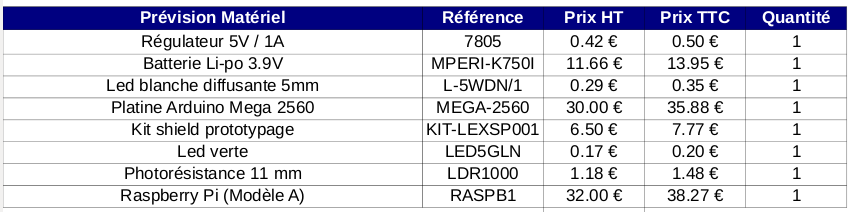
\includegraphics[width=550px]{images/lextronic.png}
		\caption{Bon de commande}
	\end{figure}


	\part{Bilan et conclusion}
	\chapter{Conclusion}
	La réalisation de ce projet d'électronique nous a permis tout d'abord d'acquérir des compétences dans de multiples domaines : l'électronique, la programmation et le réseau. Nous avons dû faire appel à de nombreuses connaissances et nous avons effectué de nombreuses recherches pour pouvoir réaliser l'évolution du réveil intelligent, particulièrement en électronique pour la Raspberry et la Arduino.\\

Bien que nous étions à travailler en groupe avec les précédents projets que nous avons pu réalisé lors de notre scolarité à l'INSA, ce projet a été différent car pour la première fois nous devions rendre un objet au terme du projet.\\

La partie qui nous a demandé le plus de travail a été l'interaction entre les différentes parties de notre projet : l'interface web de configuration, le système d'exploitation de la Raspberry ainsi que la communication entre la Raspberry et la Arduino.\\

Bien que notre projet puisse être amélioré et que celui ne soit absolument pas présentable en tant que réveil intelligent complet, nous sommes satisfaits du travail que nous avons fourni car nous avons rencontré divers obstacles avant d'arriver au résultat actuel.


	\part{Annexes}

\end{document}